

\section{An overview on the search and the best-fit template }
%Generally, a GW signal from a CBC event is expected to be buried in the detector noise and a careful data analysis needs to be performed to extract the information of the signal from the detector data. Multiple GW search pipelines are developed, equipped with various algorithms and techniques to detect the GW signal from the detector data \cite{GSTLAL1,GSTLAL2,Canton:2014ena,Usman:2015kfa,Nitz:2017svb}.  

%introducing search pipelines. 
In the second generation detectors, a GW signal from CBC events are buried in the detector noise and a careful data analysis needs to be performed to extract the information of the signal from the detector data. Several GW search pipelines have been developed, equipped with various algorithms and techniques to detect the GW signal from the detector data \cite{burstpipeline, GSTLAL1,GSTLAL2,Canton:2014ena,Usman:2015kfa,Nitz:2017svb}.  


%INTRODUCING TERMS
The search for GW from CBCs relies on a  technique known as \textit{matched filtering} \cite{SchutzBF, JCreightonBook}. The basic idea in match filtering is to compare the data from the detector to the expected GW waveform. These expected GW waveforms are, known as templates. The waveforms are obtained by solving the Einsteins equation, either using a variety of analytical approximations or numerically or with a combination of both analytical and numerical techniques \cite{BH-GW-NR}.  Each method of solving Einstein's equation to obtain the templates corresponds to a \textit{waveform family} or an \textit{approximant}.


%In this chapter, the specific GW search pipeline we refer to is called \textbf{$\texttt{PyCBC}$}, which is an open source software package that has inbuilt algorithms to detect and analysis CBC events from the calibrated detector data. For the details of $\texttt{PyCBC}$ search pipeline refer to \cite{Usman:2015kfa}. The search relies on a  technique known as \textit{matched filtering} \cite{SchutzBF, JCreightonBook}. The basic idea in match filtering is to `match' (or compare) the data from the detector to the expected GW waveform. These expected GW waveforms are, often times, referred to as templates. The waveforms are obtained by solving the Einsteins equation, either using a variety of analytical approximations or numerically or with a combination of both analytical and numerical techniques \cite{BH-GW-NR}.  Each variant of obtaining the templates corresponds to a \textit{waveform family} or an \textit{approximant}.

The operation of match filtering can be written down as a weighted inner product in the frequency domain,
\begin{align}
\label{eq:match}
\mathcal{M}(t) = \left\langle s| h \right\rangle = 4 \mathrm{Re} \int^{f_{high}}_{f_{low}} \frac{s(f) h^{*}(f) e^{2 \pi \iota f t}}{S_{n}(f)} df,
\end{align}
where, $s(f)$ is the Fourier transform of the data and h(f) is the template in the Fourier domain. $S_{n}(f)$ is the one-sided power spectral density (PSD) of the detector and encodes the sensitivity of the detector across the frequency band. It is computed by averaging over the detector noise realization. 
\begin{align}
\left\langle s(f)s(f') \right\rangle = \frac{1}{2} S_{n}(f) \delta(f-f') 
\end{align}

In practice, the detector data contains noise transients and is non-gaussian, and therefore additional statistical tools need to be implemented to construct a detection statistic. The detection statistic used for CBC events in $\texttt{PyCBC}$ is called chi-square-weighted-new SNR details of which can be found in \cite{newSNR1,newSNR2,FindChirp,Usman:2015kfa} . 


When a GW signal from a CBC event is present in the data, one does not a priori know the parameters of the compact binary system. Therefore, a bank of templates is created and the data is matched against each of the templates present in this bank \cite{FindChirp}. In the search pipeline, $\texttt{PyCBC}$, the template bank corresponds to waveforms emitted by the compact binary systems whose component masses have spins that are aligned/anti-aligned to the orbital angular momentum of the system (the bank is thus called an aligned spin bank). Further, the binaries are assumed to have negligible eccentricity. When constructing the template bank, one needs to sample the astrophysical parameter space sufficiently densely to be able to capture the GW signal with enough SNR but also keep the bank sparse enough so that it is computationally efficient. In $\texttt{PyCBC}$, the template bank is generated such that no more than 3\% SNR is lost due to the discreteness of the template bank. When a match filter operation is performed throughout this bank, the search pipeline reports the parameters of the template that produced the maximum match as the \textit{best-fit-template}. These parameters give an approximate estimate of the astrophysical parameters of the source but a further careful parameter estimation(PE) study is followed to infer the true parameters of the system. Note that the best-fit template parameters will depend on the state of the detectors at the time of the event, on the family of templates being used and the discreteness of the bank chosen. 

\section{On the detection of GW150914}

On 14th September 2015, both the LIGO detectors recorded a GW signal consistent with what GR would predict when two BHs with masses $\sim 36\Msun$ and $29\Msun$ inspiraled and merged \cite{gw150914detection,gw150914search}. The signal was first found by the Generic transient search pipeline \cite{burstpipeline,burstpipeline1}  which identifies the events by looking at the coincident exess power in the time-frequency plots of the data from the two detectors. The signal was also reported by two independent CBC focused search pipelines.  In this chapter, the specific CBC-focused GW search pipeline we refer to is called \textbf{$\texttt{PyCBC}$}, which is an open source software package that has inbuilt algorithms to detect and analysis CBC events from the calibrated detector data. For the details of $\texttt{PyCBC}$ search pipeline refer to \cite{Usman:2015kfa}.

For reporting the statistical confidence of this detection, data from a total coincident observation time of $16$ days \footnote{This the duration of coincident data obtained after applying the data quality vetoes. The details of data quality checks and vetoes applied for the analysis of GW150914 event can be found in \cite{gw150914vetos1,gw150914vetos2}}  was used for the analysis. From this data, a noise background equivalent to 608000 years was produced by performing unphysical time delay; the time shifts greater than 10 milliseconds (greater light travel time between the detector) ensure that the simulated data stream has no real astrophysical signal in it and contains only detector noise realization. The statistic used by the LIGO collaboration for detection is an empirically re-weighted combined new SNR detail of which can be found in \cite{detectionStat1}. On analyzing the data containing the GW150914 event, it was found that this event has a combined SNR of 23.6. The false alarm probability was calculated to be $\sim 2 \times 10^{ -7}$, which affirms that the signal corresponded to an astrophysical source. The statistical significance of this event was reported to be 5.1 $\sigma$. It should be emphasized that this event was exceptionally loud. 






%On 14th September 2015, both the LIGO detectors recorded a GW signal consistent with what GR would predict when two BHs with masses $\sim 36\Msun$ and $29\Msun$ inspiraled and merged \cite{gw150914detection,gw150914search}. $\texttt{PyCBC}$ was one of the search pipelines employed by the LIGO collaboration to detect the signal. For reporting the statistical confidence of this detection, data from a total coincident observation time of $16$ days \footnote{This the duration of coincident data obtained after applying the data quality vetoes. The details of data quality checks and vetoes applied for the analysis of GW150914 event can be found in \cite{gw150914vetos1,gw150914vetos2}}  was used for the analysis. From this data, a noise background equivalent to 608000 years was produced by performing unphysical time delay; time shifts greater than 10 milliseconds (greater light travel time between the detector) ensure that the simulate data stream has no real astrophysical signal in it and contains only detector noise realization. The statistic used by the LIGO collaboration for detection is an empirically re-weighted combined new SNR detail of which can be found in \cite{detectionStat1}. On analyzing the data containing the GW150914 event, it was found that this event has a combined SNR of 23.6. The false alarm probability was calculated to be $\sim 2 \times 10^{ -7}$, which affirms that the signal corresponded to an astrophysical source and is unlikely to be a noise mimicker. The statistical significance of this event was reported to be 5.1 $\sigma$. It should be emphasized that this event was exceptionally loud. 

%Further, in Table \ref{tab:best-fitGW150914}, we list the best-fit parameters reported by the $\texttt{PyCBC}$ search. It should be reiterated that these parameters are approximate parameters but they are obtained in low latency; therefore, these values were used to perform preliminary analysis of the event. The values of best-fit-template parameter reported by the search differ from the parameters inferred on performing a careful Bayesian parameter estimation (compare Table \ref{tab:best-fitGW150914} with results presented in papers \cite{gw150914PE}). 




The $\texttt{PyCBC}$ search pipeline, also reports the parameters of the best-fit-template and therefore, provides a rough estimate of the astrophysical parameters of the system immediately after identifying the event.  In Table \ref{tab:best-fitGW150914}, we list the best-fit parameters reported by the $\texttt{PyCBC}$ search for the GW150914 event. It should be noted that the values of best-fit-template parameters reported by the search differ from the parameters inferred on performing a Bayesian parameter estimation (compare Table \ref{tab:best-fitGW150914} with results presented in papers \cite{gw150914PE}). However, the parameter estimation studies take a longer timescale (order of a few weeks). The study presented in section \ref{sec:dirrect-comparision} was performed shortly after the GW150914 trigger was recorded. At that time, the parameter estimation studies were still being performed and the PE inferred values were not available. Therefore, in the study presented in section \ref{sec:dirrect-comparision}, we use the best-fit-template parameters presented in Table \ref{tab:best-fitGW150914} reported by the $\texttt{PyCBC}$ search pipeline.



\begin{table*}
\centering
\begin{tabular}{|c|c| }
\hline
Parameters 		 & Best-fit value \\ \hline
mass 1                   & 49.9 $\Msun$       \\ 
mass 2                   & 36.6 $\Msun$         \\
spin 1z                  & 0.96          \\ 
spin 2z                  & -0.89         \\ \hline
Effective Distance in L1 & 1194.9118 Mpc \\ 
Effective Distance in H1 & 970.70534 Mpc \\  \hline
Arrival Phase in L1      & 0.58 rad      \\ 
Arrival Phase in H1      & -2.77 rad     \\ \hline
\end{tabular}
\caption{The parameters of the best-fit-template for GW150914 trigger reported by the $\texttt{PyCBC}$ search pipeline obtained by analyzing the data containing GW150914 trigger. These values are used in our study presented in section \ref{sec:dirrect-comparision}}.
\label{tab:best-fitGW150914}
\end{table*}


\section{Direct comparison of the data and best fit template}
\label{sec:dirrect-comparision}
The exceptionally loud nature of GW150914 trigger prompted exploration of the raw data from the detectors directly. In this study, we present the first visualization of the GW150914 event directly from the raw data from the LIGO detectors. The premise of this work is to visually inspect that the signal seen by the LIGO instruments at Hanford site (H1) and the Livingston site (L1) are consistent with each other, i.e, the data from each of the detectors can be lined up against each other. We also check that the data from the detectors are consistent with the best-fit-template parameters reported by the search pipeline, thereby ensuring that both the detectors see the same astrophysical signal. 


The raw GW strain seen by the LIGO detectors are recorded in a channel called the $\texttt{GDS-CALIB-STRAIN}$. The data in this channel is calibrated but no other data quality vetoes are applied. We use the timeseries recorded in this channel from both the detectors and perform a minimal set of filtering needed to visually inspect the GW event in the data.

To compare the data from the two detectors, we first condition the data such that the unphysical artefacts that are introduced due to detectors configurations are removed.  The sensitivity of the detectors are not uniform across all frequencies in its band; the sensitivity of the detector as a function of the frequencies is encoded in the detector PSD. Also, each detector in the network can have a different detector PSD depending on the state of the instrument and this also could vary with time. To remove this feature from the data, we `whiten' it;  the data from each of the detectors is Fourier transformed and is divided by the respective detector's inverse noise amplitude spectrum in the Fourier domain. 

The data is band-passed to remove contaminants in frequencies that the detector is not sensitive to.  There are also known physical mechanisms in the detectors that produce narrow frequency but high amplitude noise contamination in the detector data (for example, harmonics of electricity power line, harmonics of the resonance frequency of mirror suspensions etc). In order to see the signal, we have to notch out these contaminated frequencies bands from the data. We do this using an analytical filter constructed using a zero-pole-gain (zpk-filter) model that notches out the power-line frequencies. The filter is depicted in the bottom right inlay panel of Figure \ref{fig:overlayGW150914}. The filter is designed such that the amplitude is set to 1 at 100 Hz. Next, the data is filtered both forward and then backwards to ensure that filtering does not introduce a phase error (zero-phase filtering).  Note that the filter is acausal (specifically, symmetric in time) and is designed to introduce a zero-phase offset. The impulse response of the filter can be seen in the top right inlay panel of Figure \ref{fig:overlayGW150914}. At this point, it must be emphasized that these sets of filtering are very non-aggressive and are the minimal data conditioning that we had to perform in order to visually examine the data. 




%The exceptionally loud nature of GW150914 trigger prompted us to look at the raw data from the detectors directly, unlike in the case of search pipelines where one is more concerned about the SNR timeseries for the events.  In this section, we describe our preliminary analysis on the raw data containing the GW150914 trigger.  The basic premise of this work was to check for visual consistency between the observed signal and the best-fit template reported by the search pipeline.

%The raw GW strain seen by the LIGO detectors are recorded in a channel called the $\texttt{GDS-CALIB-STRAIN}$. The data in this channel is calibrated but no other data quality vetoes are applied. We use the timeseries recorded in this channel and perform a minimal set of filtering needed to visually see the GW event. Firstly, the sensitivity of the detectors are not uniform across all frequencies in its band and the sensitivity to frequencies is encoded in the PSD.  Therefore, to remove this feature, we `whiten' the data by applying an inverse noise amplitude spectrum to the data in the Fourier domain.  Moreover, the data needs to be band passed to remove contaminants in frequencies that the detector is not sensitive to. Furthermore, the detector data contains known noise contaminations that are localized in frequencies. One such noise contamination comes due to the electric power line and is localized at frequencies that are harmonics of 60 Hz. In order to see the signal, we have to notch out these power-line frequencies from the data. We do this using an analytical filter constructed using a zero-pole-gain (zpk-filter) model that notches out the power-line frequencies. The filter is depicted in the bottom right inlay panel of Figure \ref{fig:overlayGW150914}. The filter is designed such that the amplitude is set to 1 at 100 Hz. Next, the data is filtered both forward and then backwards to ensure that filtering does not introduce a phase error (zero-phase filtering).  Note that the filter is acausal (specifically, symmetric in time) and is designed to introduce a zero-phase offset. The impulse response of the filter can be seen in the top right inlay panel of Figure \ref{fig:overlayGW150914}. At this point, it must be emphasized that these sets of filtering are very non-aggressive and are the minimal data conditioning that we had to perform in order to visually examine the data. 

From the search pipeline, we find the time at which the SNR peaks in each of the detector data. This corresponds to the time when the template aligns best with the data. However, note that the  value of this time-stamp may vary slightly when the search is performed using the different template families (also known as waveform approximants); they depend on the convention of defining the $t_{merger}$ within the waveform family.We find that this difference in the time-stamps can affect the alignment of the template with the data. 

To overlay the best-fit template on to the detector data timeseries, we need a time-domain template with the best-fit-template parameters. However, typically the search uses a frequency domain template in order to increase computational efficiency. We construct a template bank consisting of a single time-domain template corresponding to the parameter described in Table \ref{tab:best-fitGW150914}. The template family used in our study corresponds to a spinning effective one body waveform (called the $\texttt{SEOBNRv2}$ approximant in the $\texttt{LAL}$ code library)  \cite{SEOBNRv2}. We then perform a search on the data containing the event using this single-template template bank and record the reported time of the merger. This reported time of merger is used to align the raw data from the two detectors. This is also used to align the best-fit template to the data to produce the overlay plot presented in Figure \ref{fig:overlayGW150914}. The merger times obtained are listed below in Table \ref{tab:arrival-time}.


\begin{table}[]
\centering
\begin{tabular}{|c|c|}
\hline
Detector & Time-stamp (in sec)        \\ \hline
L1       & 1126259462.415039062 \\
H1       & 1126259462.422363281 \\ \hline
\end{tabular}
\caption{The time at which SNR timeseries peaks in each of the detector. The detector data is matched to a time-domain template, $\texttt{SEOBNRv2}$, corresponding to the best-fit-template parameters reported by the $\texttt{PyCBC}$ search.}
\label{tab:arrival-time}
\end{table}

This corresponds to a time delay of 7.32 ms between the Livingston (L1) and Hanford (H1) detectors. Our analysis uses a sampling rate of 16384 Hz and therefore, to align the data from the two detectors, we shift the raw data of H1 by 120 sample points. Also, the two detectors see signal arriving with different phase as their location and orientation are different. Therefore, the data is appropriately phase shifted by the values presented in Table \ref{tab:best-fitGW150914} to obtain alignment presented in Figure \ref{fig:overlayGW150914}.

\begin{figure*}
\subfloat{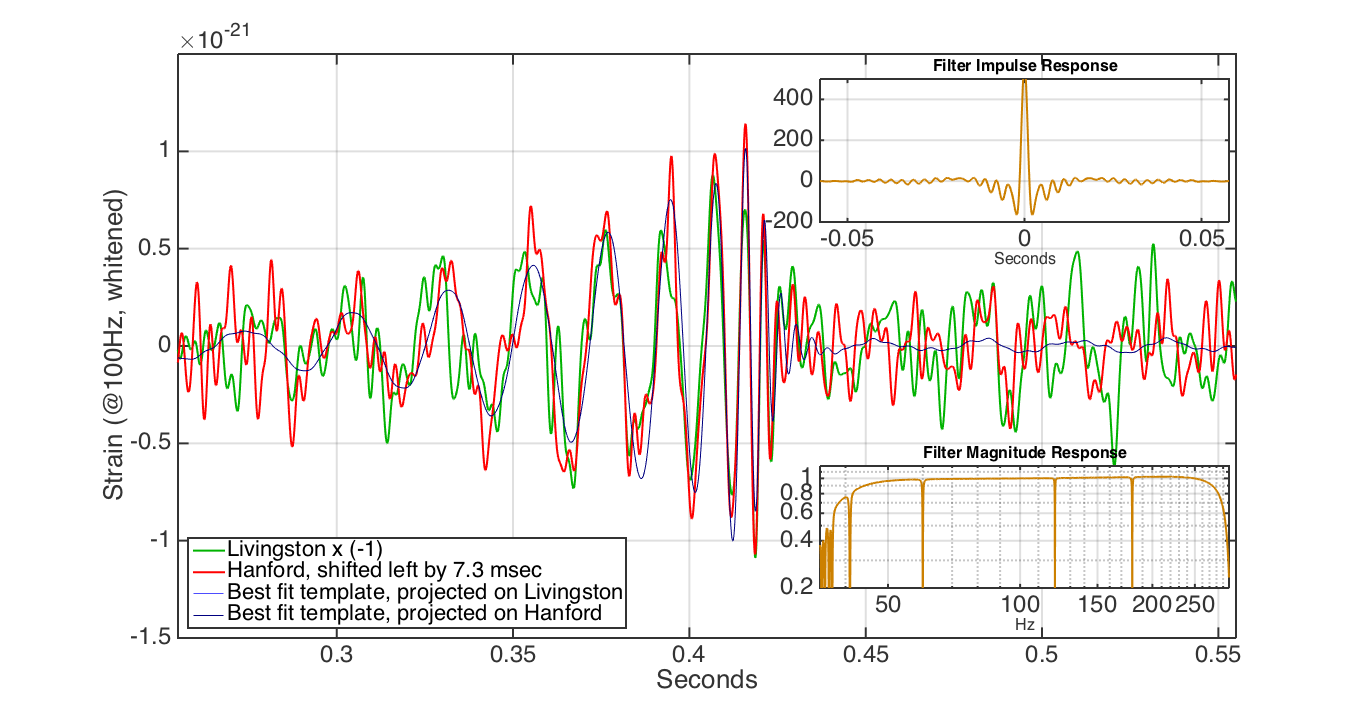
\includegraphics[width=\textwidth]{figures/overlayGW150914.png} }
\caption{Direct comparison of the detector data with the best fit template. The data from the H1 and L1 have been minimally filtered and  appropriately shifted to align with each other. The best fit template corresponding to each of the detector timeseries is overlayed on the data. The inlay panel display the details of the filters used to condition the data}
\label{fig:overlayGW150914}
\end{figure*}

The result of this study is presented in Figure \ref{fig:overlayGW150914}. We see an excellent agreement between the raw data from the two detectors (see the coherence in the green and the red curve in the main panel). Furthermore, note that the best-fit-template (the thin blue and black lines) match very well with the two detector data (and with each other). In this plot we see that a minimal set of non-aggressive filtering allows us to clearly see the inspiral and merger phase of the GW signal buried in the detector noise. However, the ringdown portion of the waveform is buried under the noise floor. 

A refined version of Figure \ref{fig:overlayGW150914} was prepared by the LIGO collaboration and is presented in the top two panels of Figure 1 in the GW150914 detection paper \cite{gw150914detection}. For the easy of comparison, we present this plot in Figure \ref{fig:Fig1GW150914detection}. Figure \ref{fig:Fig1GW150914detection} differs from Figure \ref{fig:overlayGW150914} in the following ways. The template that was used in the making of Figure 1 of \cite{gw150914detection} used the numerical relativity (NR) waveform from the SXS-NR waveform catalog indexed as SXS:BBH:0305. Note that this waveform also does not correspond to the most-likely or  maximum a posteriori parameters reported by the parameter estimation presented in \cite{gw150914PE} and  \cite{gw150914PEseobnrv3}. However, it produces a overlap of 0.993 with the maximum a posteriori parameters reported in \cite{gw150914PEseobnrv3}. Further, template amplitude, phase, and arrival time are obtained by minimize the visual content of the residuals. Furthermore, for data conditioning a Butter-worth bandpass filter from 35.0 Hz to 350.0 Hz was applied followed by notching out frequencies where the PSD spiked. 

\begin{figure*}
\subfloat{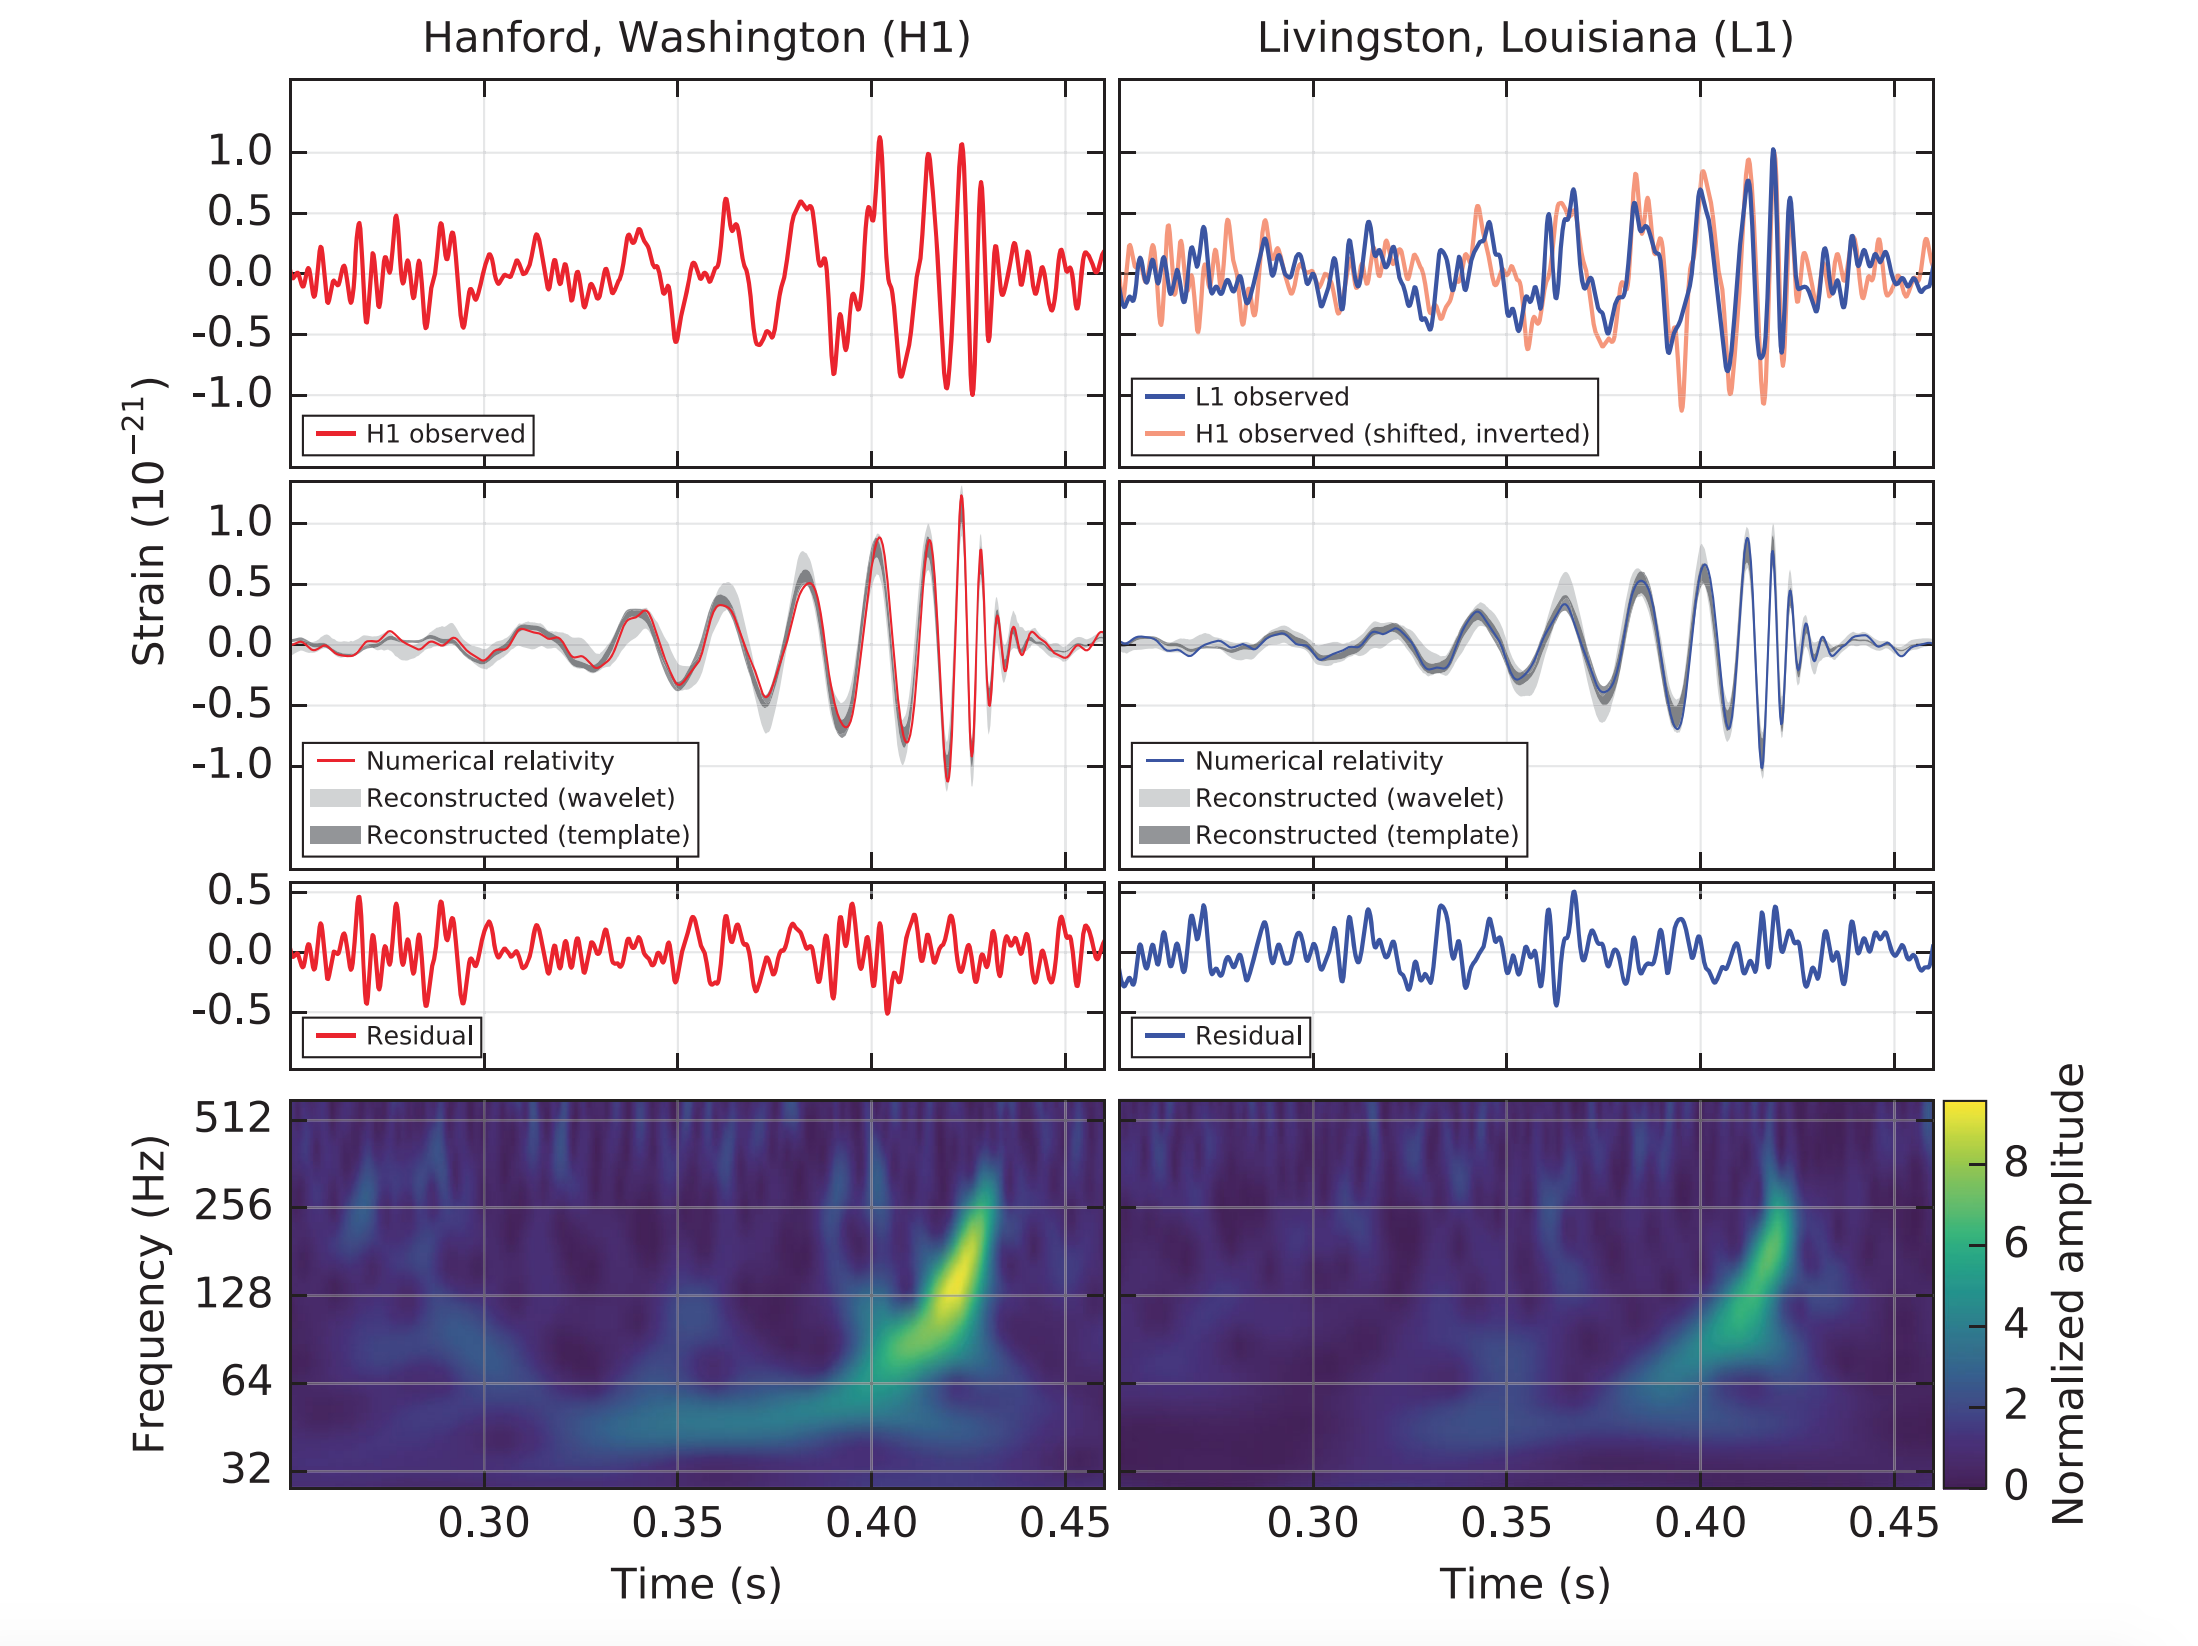
\includegraphics[width=\textwidth]{figures/dectionPaperFig1.png} }
\caption{Figure 1 from GW150914 detection paper \cite{gw150914detection} . This Figure is taken from the GW150915 detection paper \cite{gw150914detection} by the LIGO collaboration. The top two panels of this Figure shows a more refined versino of the plot we produce in our preliminary study presented in Figure \ref{fig:overlayGW150914}.}
\label{fig:Fig1GW150914detection}
\end{figure*}0

\section{Parameters of GW150914 inferred using SEOBNRv3 waveform family}

%Having emphasized that the parameters reported by the search are approximate and a careful PE needed to be followed in order to estimate the astrophysical parameters, in this section we briefly summarize the parameters estimate for GW150915 using a template family that models spinning and precessing BBH waveforms in an effective one body formulation. This section contains results of the PE studies performed by the LIGO collaboration that are presented in papers \cite{gw150914PE} and \cite{gw150914PEseobnrv3}.  

Since the parameters reported by the search are approximate, a Bayesian PE needed to be followed in order to estimate the astrophysical parameters. In this section, we summarize the parameters estimate for GW150915 using a template family that models spinning and precessing BBH waveforms in an Effective One Body (EOB) formulation. This section contains results of the PE studies performed by the LIGO collaboration that are presented in papers \cite{gw150914PE} and \cite{gw150914PEseobnrv3}.



%PE of GW150914 was initially performed using two template families that had independent ways of computing the waveforms \cite{gw150914PE}. The two template families were a) One of the template families used was based on an effective one body (EOB) formulation and is calibrated to a set of numerical relativity simulation. This model did not allow for a non-aligned spin, thereby did not contain precession physics in the waveform modeling. In the $\texttt{LAL}$ code library, the implementation of this template family is called $\texttt{SEOBNRv2}$  \cite{SEOBNRv2}. Further, to perform the PE study present in \cite{gw150914PE}, an implementation of the reduced ordered model of this waveform in the frequency domain, called the $\texttt{SEOBNRv2-ROM-DoubleSpin}$,  was used in view of computational efficiency.  b) The second waveform family used in the PE study presented in \cite{gw150914PE}, models the waveform by phenomenologically predicting the amplitude and phase evolution.  This waveform family is also calibrated to a set of numerical relativity simulations. Furthermore, in this waveform family, the precession physics of the binary system is incorporated (i.e) it can generate waveform corresponding to non-aligned binary black hole systems.  In the $\texttt{LAL}$ code library,  the implementation of this waveform family is called as $\texttt{IMRPhenomPv2}$  \cite{IMRPhenomPv2}. 

PE of GW150914 was initially performed using two template families that had independent ways of computing the waveforms \cite{gw150914PE}.
\begin{enumerate}
\item One of the template families used was based on an effective one body (EOB) formulation and is calibrated to a set of numerical relativity simulation. This model did not allow for a non-aligned spin, thereby did not contain precession physics in the waveform modelling. In the $\texttt{LAL}$ code library, the implementation of this template family is called $\texttt{SEOBNRv2}$  \cite{SEOBNRv2}. Further, to perform the PE study present in \cite{gw150914PE}, an implementation of the reduced ordered model of this waveform in the frequency domain, called the $\texttt{SEOBNRv2-ROM-DoubleSpin}$,  was used in view of computational efficiency. 
\item The second waveform family used in the PE study presented in \cite{gw150914PE}, models the waveform by phenomenologically predicting the amplitude and phase evolution.  This waveform family is also calibrated to a set of numerical relativity simulations. Furthermore, in this waveform family, the precession physics of the binary system is incorporated (i.e) it can generate waveform corresponding to non-aligned binary black hole systems.  In the $\texttt{LAL}$ code library,  the implementation of this waveform family is called as $\texttt{IMRPhenomPv2}$  \cite{IMRPhenomPv2}. 
\end{enumerate}

 

%he primary reason that the LIGO collaboration performed the PE studies of the GW150914 event using two independent template families was to understand the effect of waveform systematics in the inferred astrophysical parameters of the system \cite{gw150914PE}. It was then anticipated that the difference in the inferred parameters arising due to the difference in the waveform family will be on the pessimistic end, as we a priori know that $\texttt{SEOBNRv2}$ lacks the precision physics in it. Therefore, an implementation of effective one body template family that incorporated the precession physics was developed shortly after the initial parameter estimation analysis presented in \cite{gw150914PEseobnrv3}. The new implementation of precessing EOB waveform family was called $\texttt{SEOBNRv3}$  and the details of the physics in modeling this waveform can be found in \cite{SEOBNRv3}. I was involved in the review process of the implementation of this waveform family in the $\texttt{LAL}$ code library.  Table \ref{tab:PEwithSEOBNRV3} presents the parameter estimation results obtained by the LIGO collaboration using the $\texttt{SEOBNRv3}$ template family. It was found that the inferred parameters of GW150914 using the two precision models were indeed very close, affirming that inferred astrophysical parameters of the system are not affected significantly by the difference in the waveform models. Further, the difference in inferred astrophysical parameters due the difference in waveform family used for performing the PE study is beautifully visualized in Figure 1 of \cite{gw150914PEseobnrv3}. 

Two independent template families were to understand the effect of waveform systematics in the inferred astrophysical parameters of the system \cite{gw150914PE}. It was then anticipated that the difference in the inferred parameters arising due to the difference in the waveform family will be on the pessimistic end, as we a priori know that $\texttt{SEOBNRv2}$ lacks the precision physics in it. An implementation of effective one body template family that incorporated the precession physics was developed shortly after the initial parameter estimation analysis presented in \cite{gw150914PEseobnrv3}. The new implementation of precessing EOB waveform family was called $\texttt{SEOBNRv3}$  and the details of the physics in modelling this waveform can be found in \cite{SEOBNRv3}. Table \ref{tab:PEwithSEOBNRV3} presents the parameter estimation results obtained by the LIGO collaboration using the $\texttt{SEOBNRv3}$ template family. It was found that the inferred parameters of GW150914 using the two precision models were indeed very close, affirming that inferred astrophysical parameters of the system are not affected significantly by the difference in the waveform models. Further, the difference in inferred astrophysical parameters due the difference in waveform family used for performing the PE study is beautifully visualized in Figure 1 of \cite{gw150914PEseobnrv3}. 





\begin{table*}
\begin{tabular}{|c|c|}
\hline
& precessing EOBNR \\
\hline
Detector-frame total mass $M/\Msun$ & $71.6^{+4.3}_{-4.1}$ \\
Detector-frame chirp mass $\mathcal{M}/\Msun$ & $30.9^{+2.0}_{-1.9}$ \\
Detector-frame primary mass $m_1/\Msun$ & $38.9^{+5.1}_{-3.7}$  \\
Detector-frame secondary mass $m_2/\Msun$ & $32.7^{+3.6}_{-4.8}$  \\
Detector-frame final mass $M_\mathrm{f}/\Msun$ & $68.3^{+3.8}_{-3.7}$ \\ \hline
Source-frame total mass $M^{\mathrm{source}}/\Msun$ & \
$65.6^{+4.1}_{-3.8}$ \\
Source-frame chirp mass $\mathcal{M}^{\mathrm{source}}/\Msun$ & \
$28.3^{+1.8}_{-1.7}$ \\
Source-frame primary mass $m_1^{\mathrm{source}}/\Msun$ & \
$35.6^{+4.8}_{-3.4}$ \\
Source-frame secondary mass $m_2^{\mathrm{source}}/\Msun$ & \
$30.0^{+3.3}_{-4.4}$ \\
Source-frame final mass $M_\mathrm{f}^{\mathrm{source}}/\Msun$ & \
$62.5^{+3.7}_{-3.4}$\\
 \hline
Mass ratio $q$ & $0.84^{+0.14}_{-0.20}$ \\
\hline
Effective inspiral spin parameter $\chi_\mathrm{eff}$ \
&$-0.02^{+0.14}_{-0.16}$  \\
Effective precession spin parameter $\chi_\mathrm{p}$ \
&$0.28^{+0.38}_{-0.21}$  \\
Dimensionless primary spin magnitude $a_1$ &$0.22^{+0.43}_{-0.20}$ \\
Dimensionless secondary spin magnitude $a_2$ &$0.29^{+0.52}_{-0.27}$  \\
Final spin $a_\mathrm{f}$ &$0.68^{+0.05}_{-0.05}$ \\
 \hline
Luminosity distance $D_\mathrm{L}/\mathrm{Mpc}$ &$440^{+160}_{-180}$ \\
Source redshift $z$ &$0.094^{+0.032}_{-0.037}$ \\
\hline
Upper bound on primary spin magnitude $a_1$ & 0.54\\
Upper bound on secondary spin magnitude $a_2$ & 0.70\\
Lower bound on mass ratio $q$ & 0.69 \\ \hline
\end{tabular}
\caption{This Table presents the parameters of GW150914 estimated by the LIGO collaboration using the fully precessing EOB templates. This Table contains the first two columns presented in Table 1 of \cite{gw150914PEseobnrv3}. In the Table the median value is quoted along with the 90\% credible intervals.}
\label{tab:PEwithSEOBNRV3}
\end{table*}
